\newpage
\phantomsection
{\centering \section*{PHỤ LỤC}}
\addcontentsline{toc}{section}{PHỤ LỤC}

% Cấu hình đánh số riêng cho hình vẽ và bảng biểu trong Phụ lục
\setcounter{figure}{0}
\renewcommand{\thefigure}{PL.\arabic{figure}}
\setcounter{table}{0}
\renewcommand{\thetable}{PL.\arabic{table}}

\subsection*{HẠN CHẾ TÀI NGUYÊN}

Là một dự án cá nhân,
hệ thống hiện tại đang gặp phải những
hạn chế
về mặt hạ tầng và chi phí tài nguyên.
Cụ thể, việc triển khai Kong API Gateway
trên nền tảng miễn phí của Render (cold start),
kết hợp với giới hạn
băng thông network của VPS
và hạn mức LLM, đã tạo ra những nút thắt cổ chai đáng kể về hiệu năng.
Việc áp dụng mẫu Outbox có ưu điểm lớn là kiến trúc đơn giản,
dễ triển khai
nhưng lại bộc lộ nhược điểm chí mạng là liên tục thực hiện truy vấn (polling) vào database ngay cả khi không có dữ liệu thay đổi.
Điều này vô tình gây áp lực cực kỳ lớn lên cấu hình phần cứng vốn đã khiêm tốn của database postgres (chạy trên cluster miễn phí của Neon).
Do phân khúc tài nguyên bị thắt chặt và hệ thống hiện tại vẫn chưa tích hợp phần kiểm thử hiệu năng (Performance Testing) để đo lường định lượng, dự án vẫn chưa thể đạt đến trạng thái tối ưu và hoạt động mượt mà như kỳ vọng.

% \subsection*{Bảng thông tin các trường hợp kịch bản}

\subsection*{TRƯỜNG HỢP KỊCH BẢN}

Dưới đây là bảng thống kê kết quả chạy thử nghiệm tự động các kịch bản
để đánh giá khả năng chống ảo giác (hallucination), độ chính xác của tài liệu truy xuất (context) và hiệu năng phản hồi (latency) của hệ thống.
Bảng dữ liệu
này
được chạy tự động
với Github Actions.

\textbf{Link:} \url{https://github.com/20206205Tech/demo/actions/runs/28315626225}

\begin{figure}[H]
\centering
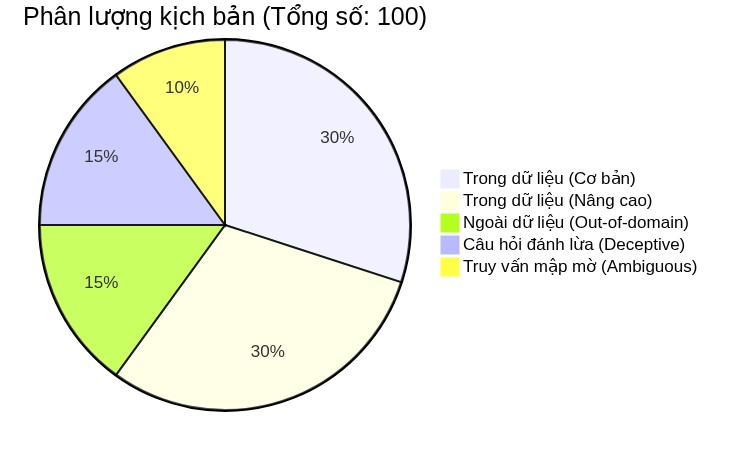
\includegraphics[width=0.85\textwidth]{contents/0/phu_luc/python/bang3.png}

\refstepcounter{figure}
\textbf{Hình \thefigure:} Biểu đồ phân lượng các kịch bản thử nghiệm hệ thống
\label{fig:ti_le_kich_ban_thu_nghiem}
\end{figure}


\begin{longtable}{|l|p{6.5cm}|c|c|}
\caption{Bảng thống kê các kịch bản thử nghiệm hệ thống} \label{tab:thong_ke_chi_tiet} \\
\hline
\makecell[l]{\textbf{Phân loại}\\\textbf{trường hợp}} & \textbf{Câu hỏi} & \makecell{\textbf{Tài liệu}\\\textbf{truy xuất}} & \textbf{Thời gian} \\ \hline
\endfirsthead
\multicolumn{4}{c}{{\bfseries Bảng \thetable{} -- Tiếp theo từ trang trước}} \\
\hline
\makecell[l]{\textbf{Phân loại}\\\textbf{trường hợp}} & \textbf{Câu hỏi} & \makecell{\textbf{Tài liệu}\\\textbf{truy xuất}} & \textbf{Thời gian} \\ \hline
\endhead
\hline
\multicolumn{4}{r}{{Tiếp tục ở trang sau}} \\
\endfoot
\hline
\endlastfoot
\makecell[l]{Trong dữ liệu\\(Cơ bản)} & Thời gian thử việc tối đa đối với người lao động có trình độ đại học là bao lâu? & 44 tài liệu & 64.58s \\ \hline
\makecell[l]{Trong dữ liệu\\(Cơ bản)} & Thời gian thử việc tối đa của lao động có trình độ cao đẳng là bao lâu? & 26 tài liệu & 25.68s \\ \hline
\makecell[l]{Trong dữ liệu\\(Cơ bản)} & Người lao động được nghỉ bao nhiêu ngày phép năm nếu làm đủ 12 tháng trong điều kiện bình thường? & 26 tài liệu & 39.67s \\ \hline
\makecell[l]{Trong dữ liệu\\(Cơ bản)} & Lương thử việc tối thiểu bằng bao nhiêu phần trăm lương của công việc đó? & 22 tài liệu & 14.22s \\ \hline
\makecell[l]{Trong dữ liệu\\(Cơ bản)} & Thời giờ làm việc bình thường không quá bao nhiêu giờ trong một ngày và một tuần? & 0 tài liệu & 1.92s \\ \hline
\makecell[l]{Trong dữ liệu\\(Cơ bản)} & Làm thêm giờ vào ngày nghỉ hằng tuần được trả lương ít nhất bằng bao nhiêu? & 0 tài liệu & 31.91s \\ \hline
\makecell[l]{Trong dữ liệu\\(Cơ bản)} & Làm thêm giờ vào ngày nghỉ lễ, tết, ngày nghỉ có hưởng lương được trả lương ít nhất bằng bao nhiêu? & 0 tài liệu & 30.08s \\ \hline
\makecell[l]{Trong dữ liệu\\(Cơ bản)} & Có bao nhiêu loại hợp đồng lao động theo Bộ luật Lao động hiện hành? & 22 tài liệu & 55.67s \\ \hline
\makecell[l]{Trong dữ liệu\\(Cơ bản)} & Thời gian thử việc đối với công việc cần trình độ chuyên môn kỹ thuật trung cấp là bao lâu? & 23 tài liệu & 13.29s \\ \hline
\makecell[l]{Trong dữ liệu\\(Cơ bản)} & Người lao động làm việc vào ban đêm được trả thêm ít nhất bao nhiêu phần trăm tiền lương? & 0 tài liệu & 29.08s \\ \hline
\makecell[l]{Trong dữ liệu\\(Cơ bản)} & Lao động nữ mang thai từ tháng thứ mấy thì được giảm giờ làm việc hoặc chuyển công việc nhẹ hơn? & 22 tài liệu & 13.99s \\ \hline
\makecell[l]{Trong dữ liệu\\(Cơ bản)} & Người sử dụng lao động có được giữ bản chính giấy tờ tùy thân, văn bằng, chứng chỉ của người lao động không? & 22 tài liệu & 11.91s \\ \hline
\makecell[l]{Trong dữ liệu\\(Cơ bản)} & Tuổi nghỉ hưu của người lao động trong điều kiện lao động bình thường được quy định như thế nào? & 24 tài liệu & 20.74s \\ \hline
\makecell[l]{Trong dữ liệu\\(Cơ bản)} & Người lao động kết hôn được nghỉ bao nhiêu ngày và có được hưởng nguyên lương không? & 22 tài liệu & 13.34s \\ \hline
\makecell[l]{Trong dữ liệu\\(Cơ bản)} & Bố đẻ hoặc mẹ đẻ chết thì người lao động được nghỉ bao nhiêu ngày hưởng nguyên lương? & 22 tài liệu & 13.58s \\ \hline
\makecell[l]{Trong dữ liệu\\(Cơ bản)} & Con kết hôn thì người lao động được nghỉ mấy ngày và có được hưởng lương không? & 25 tài liệu & 64.10s \\ \hline
\makecell[l]{Trong dữ liệu\\(Cơ bản)} & Thời gian nghỉ thai sản của lao động nữ khi sinh con là bao lâu? & 24 tài liệu & 38.21s \\ \hline
\makecell[l]{Trong dữ liệu\\(Cơ bản)} & Khi vợ sinh con, lao động nam đang đóng bảo hiểm xã hội được nghỉ thai sản bao nhiêu ngày? & 48 tài liệu & 123.62s \\ \hline
\makecell[l]{Trong dữ liệu\\(Cơ bản)} & Người lao động làm việc bao lâu cho một người sử dụng lao động thì được tăng thêm 1 ngày phép năm? & 49 tài liệu & 24.51s \\ \hline
\makecell[l]{Trong dữ liệu\\(Cơ bản)} & Hợp đồng thử việc có bắt buộc phải đóng bảo hiểm xã hội không? & 22 tài liệu & 20.96s \\ \hline
\makecell[l]{Trong dữ liệu\\(Cơ bản)} & Người sử dụng lao động phải báo trước bao nhiêu ngày khi đơn phương chấm dứt hợp đồng lao động không xác định thời hạn? & 54 tài liệu & 37.64s \\ \hline
\makecell[l]{Trong dữ liệu\\(Cơ bản)} & Tiền lương trong thời gian nghỉ thai sản của người lao động do cơ quan nào chi trả? & 44 tài liệu & 193.33s \\ \hline
\makecell[l]{Trong dữ liệu\\(Cơ bản)} & Người lao động có được tạm ứng tiền lương khi gặp khó khăn không? & 31 tài liệu & 33.15s \\ \hline
\makecell[l]{Trong dữ liệu\\(Cơ bản)} & Bộ luật Lao động quy định những hình thức xử lý kỷ luật lao động nào? & 75 tài liệu & 50.61s \\ \hline
\makecell[l]{Trong dữ liệu\\(Cơ bản)} & Có được áp dụng nhiều hình thức xử lý kỷ luật lao động đối với một hành vi vi phạm kỷ luật không? & 22 tài liệu & 13.05s \\ \hline
\makecell[l]{Trong dữ liệu\\(Cơ bản)} & Thời hiệu xử lý kỷ luật lao động tối đa là bao lâu? & 22 tài liệu & 12.31s \\ \hline
\makecell[l]{Trong dữ liệu\\(Cơ bản)} & Người lao động bị tạm đình chỉ công việc trong những trường hợp nào? & 31 tài liệu & 21.27s \\ \hline
\makecell[l]{Trong dữ liệu\\(Cơ bản)} & Thời gian tạm đình chỉ công việc tối đa đối với người lao động là bao lâu? & 22 tài liệu & 34.35s \\ \hline
\makecell[l]{Trong dữ liệu\\(Cơ bản)} & Người lao động được nghỉ hưởng nguyên lương vào những ngày lễ, tết nào trong năm? & 29 tài liệu & 55.58s \\ \hline
\makecell[l]{Trong dữ liệu\\(Cơ bản)} & Người sử dụng lao động có phải trả lương cho ngày nghỉ phép hằng năm chưa nghỉ hết không? & 28 tài liệu & 18.42s \\ \hline
\makecell[l]{Trong dữ liệu\\(Nâng cao)} & Cách tính trợ cấp thôi việc cho người lao động làm việc từ 5 năm trở lên? & 22 tài liệu & 33.46s \\ \hline
\makecell[l]{Trong dữ liệu\\(Nâng cao)} & Trường hợp nào người sử dụng lao động được đơn phương chấm dứt hợp đồng lao động mà không cần báo trước? & 25 tài liệu & 62.60s \\ \hline
\makecell[l]{Trong dữ liệu\\(Nâng cao)} & Trợ cấp mất việc làm được tính và chi trả cho người lao động như thế nào? & 22 tài liệu & 29.90s \\ \hline
\makecell[l]{Trong dữ liệu\\(Nâng cao)} & Lao động nữ nuôi con dưới 12 tháng tuổi được hưởng những quyền lợi gì về thời giờ làm việc và nghỉ ngơi? & 46 tài liệu & 139.00s \\ \hline
\makecell[l]{Trong dữ liệu\\(Nâng cao)} & Người lao động đơn phương chấm dứt hợp đồng lao động trái pháp luật thì phải bồi thường những khoản nào? & 30 tài liệu & 21.09s \\ \hline
\makecell[l]{Trong dữ liệu\\(Nâng cao)} & Doanh nghiệp có được quyền sa thải người lao động tự ý bỏ việc 5 ngày cộng dồn trong 30 ngày không? & 22 tài liệu & 86.90s \\ \hline
\makecell[l]{Trong dữ liệu\\(Nâng cao)} & Quy trình xử lý kỷ luật sa thải người lao động cần tuân thủ những bước nào để hợp pháp? & 51 tài liệu & 181.88s \\ \hline
\makecell[l]{Trong dữ liệu\\(Nâng cao)} & Nếu doanh nghiệp đơn phương chấm dứt hợp đồng lao động trái pháp luật thì phải bồi thường những khoản nào cho người lao động? & 46 tài liệu & 82.01s \\ \hline
\makecell[l]{Trong dữ liệu\\(Nâng cao)} & Người lao động làm công việc nặng nhọc, độc hại, nguy hiểm được nghỉ bao nhiêu ngày phép năm? & 51 tài liệu & 38.91s \\ \hline
\makecell[l]{Trong dữ liệu\\(Nâng cao)} & Cách tính tiền lương làm thêm giờ vào ban đêm của ngày nghỉ lễ, tết thế nào? & 0 tài liệu & 224.41s \\ \hline
\makecell[l]{Trong dữ liệu\\(Nâng cao)} & Người sử dụng lao động có được tự ý khấu trừ lương của người lao động để bồi thường thiệt hại dụng cụ bị hư hỏng không? & 22 tài liệu & 63.24s \\ \hline
\makecell[l]{Trong dữ liệu\\(Nâng cao)} & Hợp đồng lao động đương nhiên chấm dứt trong những trường hợp nào? & 32 tài liệu & 146.65s \\ \hline
\makecell[l]{Trong dữ liệu\\(Nâng cao)} & Khi chuyển người lao động sang làm công việc khác so với hợp đồng lao động, doanh nghiệp cần tuân thủ điều kiện gì? & 26 tài liệu & 53.27s \\ \hline
\makecell[l]{Trong dữ liệu\\(Nâng cao)} & Tiền lương của người lao động trong thời gian ngừng việc do lỗi của người sử dụng lao động được tính thế nào? & 22 tài liệu & 23.55s \\ \hline
\makecell[l]{Trong dữ liệu\\(Nâng cao)} & Tiền lương ngừng việc do sự cố điện, nước hoặc thiên tai, dịch bệnh được thỏa thuận như thế nào? & 23 tài liệu & 21.71s \\ \hline
\makecell[l]{Trong dữ liệu\\(Nâng cao)} & Doanh nghiệp có bắt buộc phải thưởng Tết hay lương tháng 13 cho người lao động không? & 22 tài liệu & 191.65s \\ \hline
\makecell[l]{Trong dữ liệu\\(Nâng cao)} & Thỏa ước lao động tập thể là gì và khi nào nó chính thức có hiệu lực? & 22 tài liệu & 19.07s \\ \hline
\makecell[l]{Trong dữ liệu\\(Nâng cao)} & Trình tự, thủ tục giải quyết tranh chấp lao động cá nhân tại Hòa giải viên lao động diễn ra thế nào? & 22 tài liệu & 236.71s \\ \hline
\makecell[l]{Trong dữ liệu\\(Nâng cao)} & Người lao động nước ngoài làm việc tại Việt Nam bắt buộc phải có giấy phép lao động trong trường hợp nào? & 0 tài liệu & 900.35s \\ \hline
\makecell[l]{Trong dữ liệu\\(Nâng cao)} & Hợp đồng lao động bị coi là vô hiệu toàn bộ trong những trường hợp cụ thể nào? & 0 tài liệu & 105.30s \\ \hline
\makecell[l]{Trong dữ liệu\\(Nâng cao)} & Thẩm quyền tuyên bố hợp đồng lao động vô hiệu thuộc về cơ quan nào? & 28 tài liệu & 40.30s \\ \hline
\makecell[l]{Trong dữ liệu\\(Nâng cao)} & Tai nạn lao động được định nghĩa thế nào và doanh nghiệp phải bồi thường ra sao nếu có lỗi của người lao động? & 29 tài liệu & 106.23s \\ \hline
\makecell[l]{Trong dữ liệu\\(Nâng cao)} & Mức bồi thường tai nạn lao động của doanh nghiệp khi lỗi hoàn toàn thuộc về người sử dụng lao động? & 44 tài liệu & 26.37s \\ \hline
\makecell[l]{Trong dữ liệu\\(Nâng cao)} & Chi phí khám và điều trị tai nạn lao động cho người lao động do ai chi trả? & 22 tài liệu & 28.74s \\ \hline
\makecell[l]{Trong dữ liệu\\(Nâng cao)} & Doanh nghiệp có được ký hợp đồng lao động xác định thời hạn nhiều lần với người lao động cao tuổi không? & 31 tài liệu & 36.75s \\ \hline
\makecell[l]{Trong dữ liệu\\(Nâng cao)} & Khi nào người lao động có quyền từ chối làm thêm giờ mà không bị coi là vi phạm kỷ luật lao động? & 22 tài liệu & 11.06s \\ \hline
\makecell[l]{Trong dữ liệu\\(Nâng cao)} & Mức đóng bảo hiểm xã hội, bảo hiểm y tế, bảo hiểm thất nghiệp bắt buộc của người lao động hiện nay là bao nhiêu? & 48 tài liệu & 23.99s \\ \hline
\makecell[l]{Trong dữ liệu\\(Nâng cao)} & Người lao động bị ốm đau dài ngày được hưởng chế độ bảo hiểm xã hội như thế nào? & 51 tài liệu & 51.58s \\ \hline
\makecell[l]{Trong dữ liệu\\(Nâng cao)} & Doanh nghiệp thay đổi cơ cấu, công nghệ ảnh hưởng đến việc làm của nhiều người lao động thì phải lập phương án gì? & 22 tài liệu & 14.31s \\ \hline
\makecell[l]{Trong dữ liệu\\(Nâng cao)} & Quyền lợi ưu tiên thanh toán của người lao động khi doanh nghiệp bị phá sản hoặc giải thể là gì? & 47 tài liệu & 119.56s \\ \hline
\makecell[l]{Ngoài dữ liệu\\(Out-of-domain)} & Công thức tính lực hấp dẫn trong vật lý lượng tử là gì? & 0 tài liệu & 3.44s \\ \hline
\makecell[l]{Ngoài dữ liệu\\(Out-of-domain)} & Cách nấu món phở bò truyền thống của Hà Nội ngon chuẩn vị? & 0 tài liệu & 6.09s \\ \hline
\makecell[l]{Ngoài dữ liệu\\(Out-of-domain)} & Thủ đô của nước Úc là thành phố nào? & 0 tài liệu & 1.84s \\ \hline
\makecell[l]{Ngoài dữ liệu\\(Out-of-domain)} & Làm sao để viết một chương trình Python kết nối với CSDL MySQL? & 0 tài liệu & 7.68s \\ \hline
\makecell[l]{Ngoài dữ liệu\\(Out-of-domain)} & Tác giả của cuốn tiểu thuyết nổi tiếng 'Số Đỏ' là ai? & 0 tài liệu & 2.05s \\ \hline
\makecell[l]{Ngoài dữ liệu\\(Out-of-domain)} & Giải thích thuyết tương đối rộng của Albert Einstein một cách dễ hiểu? & 0 tài liệu & 4.31s \\ \hline
\makecell[l]{Ngoài dữ liệu\\(Out-of-domain)} & Làm thế nào để tự học đàn guitar tại nhà hiệu quả cho người mới bắt đầu? & 0 tài liệu & 4.87s \\ \hline
\makecell[l]{Ngoài dữ liệu\\(Out-of-domain)} & Các bước để đăng ký tài khoản quảng cáo trên Facebook Business? & 0 tài liệu & 4.46s \\ \hline
\makecell[l]{Ngoài dữ liệu\\(Out-of-domain)} & Tác động của biến đổi khí hậu đối với rạn san hô Great Barrier như thế nào? & 0 tài liệu & 4.11s \\ \hline
\makecell[l]{Ngoài dữ liệu\\(Out-of-domain)} & Điện thoại iPhone đầu tiên được Apple ra mắt vào năm nào? & 0 tài liệu & 1.82s \\ \hline
\makecell[l]{Ngoài dữ liệu\\(Out-of-domain)} & Hệ mặt trời của chúng ta có bao nhiêu hành tinh và tên của chúng? & 0 tài liệu & 2.53s \\ \hline
\makecell[l]{Ngoài dữ liệu\\(Out-of-domain)} & Cách điều trị bệnh cảm cúm thông thường tại nhà an toàn? & 0 tài liệu & 4.51s \\ \hline
\makecell[l]{Ngoài dữ liệu\\(Out-of-domain)} & Làm sao để chụp ảnh phong cảnh đẹp bằng điện thoại di động? & 0 tài liệu & 4.17s \\ \hline
\makecell[l]{Ngoài dữ liệu\\(Out-of-domain)} & Lịch sử hình thành và phát triển của mạng Internet toàn cầu? & 0 tài liệu & 6.03s \\ \hline
\makecell[l]{Ngoài dữ liệu\\(Out-of-domain)} & Những địa điểm du lịch nổi tiếng nhất không thể bỏ qua ở Đà Nẵng? & 0 tài liệu & 4.98s \\ \hline
\makecell[l]{Câu hỏi đánh lừa\\(Deceptive)} & Theo luật mới, sinh viên đi làm thêm không cần đóng thuế thu nhập cá nhân đúng không? & 44 tài liệu & 211.81s \\ \hline
\makecell[l]{Câu hỏi đánh lừa\\(Deceptive)} & Tôi nghe nói luật mới cấm hoàn toàn việc thử việc đối với tất cả các ngành nghề đúng không? & 0 tài liệu & 2.79s \\ \hline
\makecell[l]{Câu hỏi đánh lừa\\(Deceptive)} & Tại sao Bộ luật Lao động lại quy định người lao động tự ý nghỉ việc phải bồi thường cho công ty 100 tháng lương? & 0 tài liệu & 3.40s \\ \hline
\makecell[l]{Câu hỏi đánh lừa\\(Deceptive)} & Có đúng là doanh nghiệp không được phép sa thải nhân viên dù họ tự ý nghỉ việc bao nhiêu ngày đi nữa? & 22 tài liệu & 41.67s \\ \hline
\makecell[l]{Câu hỏi đánh lừa\\(Deceptive)} & Luật lao động mới có quy định tăng số ngày nghỉ phép năm tối thiểu từ 12 ngày lên 50 ngày không? & 0 tài liệu & 1.90s \\ \hline
\makecell[l]{Câu hỏi đánh lừa\\(Deceptive)} & Vì sao người lao động thử việc lại được trả lương gấp đôi lương chính thức theo quy định của pháp luật? & 0 tài liệu & 2.63s \\ \hline
\makecell[l]{Câu hỏi đánh lừa\\(Deceptive)} & Nghe nói người đi làm vào ngày Tết được trả lương gấp 10 lần ngày thường, điều này quy định ở điều mấy? & 48 tài liệu & 38.42s \\ \hline
\makecell[l]{Câu hỏi đánh lừa\\(Deceptive)} & Tại sao luật lại bắt buộc nhân viên nam nghỉ thai sản 6 tháng giống như nhân viên nữ khi vợ sinh con? & 0 tài liệu & 3.54s \\ \hline
\makecell[l]{Câu hỏi đánh lừa\\(Deceptive)} & Có đúng là người sử dụng lao động có quyền thu giữ chứng minh nhân dân của nhân viên để làm tin không? & 30 tài liệu & 19.48s \\ \hline
\makecell[l]{Câu hỏi đánh lừa\\(Deceptive)} & Tôi nghe nói hợp đồng lao động bằng lời nói luôn có giá trị cao hơn hợp đồng bằng văn bản, đúng không? & 64 tài liệu & 66.25s \\ \hline
\makecell[l]{Câu hỏi đánh lừa\\(Deceptive)} & Có phải người lao động dưới 18 tuổi thì hoàn toàn không được phép đi làm bất kỳ công việc nào? & 31 tài liệu & 21.35s \\ \hline
\makecell[l]{Câu hỏi đánh lừa\\(Deceptive)} & Có đúng là tiền lương thử việc chỉ được trả tối đa 10\% lương chính thức của công việc đó không? & 16 tài liệu & 40.63s \\ \hline
\makecell[l]{Câu hỏi đánh lừa\\(Deceptive)} & Tại sao luật quy định doanh nghiệp phải trả lương bằng đô la Mỹ (USD) cho người lao động Việt Nam? & 0 tài liệu & 2.52s \\ \hline
\makecell[l]{Câu hỏi đánh lừa\\(Deceptive)} & Nghe nói người lao động đơn phương chấm dứt hợp đồng đúng luật vẫn phải nộp phạt cho công ty, đúng không? & 22 tài liệu & 16.32s \\ \hline
\makecell[l]{Câu hỏi đánh lừa\\(Deceptive)} & Có đúng là người thử việc không cần phải tuân thủ nội quy lao động của doanh nghiệp? & 0 tài liệu & 3.33s \\ \hline
\makecell[l]{Truy vấn mập mờ\\(Ambiguous)} & Làm sao để đăng ký cái đó? & 0 tài liệu & 2.69s \\ \hline
\makecell[l]{Truy vấn mập mờ\\(Ambiguous)} & Cái đó được tính như thế nào? & 0 tài liệu & 2.12s \\ \hline
\makecell[l]{Truy vấn mập mờ\\(Ambiguous)} & Quy định về thời gian nghỉ? & 22 tài liệu & 13.11s \\ \hline
\makecell[l]{Truy vấn mập mờ\\(Ambiguous)} & Tôi phải làm gì khi bị phạt? & 22 tài liệu & 10.82s \\ \hline
\makecell[l]{Truy vấn mập mờ\\(Ambiguous)} & Khi nào thì được nhận tiền đó? & 0 tài liệu & 2.07s \\ \hline
\makecell[l]{Truy vấn mập mờ\\(Ambiguous)} & Thủ tục nghỉ việc thế nào? & 29 tài liệu & 46.93s \\ \hline
\makecell[l]{Truy vấn mập mờ\\(Ambiguous)} & Làm sao để được giảm giờ làm? & 0 tài liệu & 4.68s \\ \hline
\makecell[l]{Truy vấn mập mờ\\(Ambiguous)} & Công ty có được làm thế không? & 0 tài liệu & 1.86s \\ \hline
\makecell[l]{Truy vấn mập mờ\\(Ambiguous)} & Ký cái hợp đồng đó ở đâu? & 30 tài liệu & 57.60s \\ \hline
\makecell[l]{Truy vấn mập mờ\\(Ambiguous)} & Nghỉ thai sản thì thế nào? & 0 tài liệu & 2.74s \\ \hline
\end{longtable}


% \begin{table}[H]
\centering
\refstepcounter{table}
\textbf{Bảng \thetable:} Bảng thống kê hiệu năng và độ chính xác của hệ thống RAG
\label{tab:hieu_nang_do_chinh_xac}
\vspace{0.5em}
\begin{tabular}{|l|c|c|c|c|}
\hline
\textbf{Nhóm câu hỏi kiểm thử} & \makecell{\textbf{Tổng số}\\\textbf{câu hỏi}} & \makecell{\textbf{Phản hồi}\\\textbf{Đúng (\%)}} & \makecell{\textbf{Phản hồi Sai /}\\\textbf{Ảo giác (\%)}} & \makecell{\textbf{Không trả lời do}\\\textbf{không chắc chắn (\%)}} \\ \hline
Câu hỏi có trong CSDL pháp luật & 60 & 33 (55.0\%) & 12 (20.0\%) & 15 (25.0\%) \\ \hline
Câu hỏi ngoài phạm vi (đời sống, IT...) & 15 & 2 (13.3\%) & 13 (86.7\%) & 0 (0.0\%) \\ \hline
Câu hỏi phức tạp, tối nghĩa & 25 & 13 (52.0\%) & 10 (40.0\%) & 2 (8.0\%) \\ \hline
\textbf{Tổng cộng (Overall)} & \textbf{100} & \textbf{48 (48.0\%)} & \textbf{35 (35.0\%)} & \textbf{17 (17.0\%)} \\ \hline
\end{tabular}
\end{table}

\begin{table}[H]
\centering
\refstepcounter{table}
\textbf{Bảng \thetable:} Bảng thống kê độ chính xác (dùng LLM để đánh giá)
\label{tab:thong_ke_5_kich_ban}
\vspace{0.5em}
\begin{tabular}{|l|c|c|c|c|}
\hline
\makecell[l]{\textbf{Phân loại}\\\textbf{kịch bản}} & \makecell{\textbf{Tổng số}\\\textbf{câu hỏi}} & \makecell{\textbf{Phản hồi}\\\textbf{Đúng (\%)}} & \makecell{\textbf{Phản hồi Sai /}\\\textbf{Ảo giác (\%)}} & \makecell{\textbf{Không trả lời do}\\\textbf{không chắc chắn (\%)}} \\ \hline
\makecell[l]{Trong dữ liệu\\(Cơ bản)} & 30 & 16 (53.3\%) & 7 (23.3\%) & 7 (23.3\%) \\ \hline
\makecell[l]{Trong dữ liệu\\(Nâng cao)} & 30 & 17 (56.7\%) & 5 (16.7\%) & 8 (26.7\%) \\ \hline
\makecell[l]{Ngoài dữ liệu\\(Out-of-domain)} & 15 & 2 (13.3\%) & 13 (86.7\%) & 0 (0.0\%) \\ \hline
\makecell[l]{Câu hỏi đánh lừa\\(Deceptive)} & 15 & 9 (60.0\%) & 6 (40.0\%) & 0 (0.0\%) \\ \hline
\makecell[l]{Truy vấn mập mờ\\(Ambiguous)} & 10 & 4 (40.0\%) & 4 (40.0\%) & 2 (20.0\%) \\ \hline
% \textbf{Tổng cộng (Overall)} & \textbf{100} & \textbf{48 (48.0\%)} & \textbf{35 (35.0\%)} & \textbf{17 (17.0\%)} \\ \hline
\end{tabular}
\end{table}


% \newpage

% \subsection*{Bảng thống kê chi tiết}

% \subsection*{Thống kê về câu hỏi và trả lời}

% \newpage
% ==========================================
% Câu hỏi 1: Thời gian thử việc
% ==========================================
% \vspace{1em}
\noindent\textbf{Câu hỏi:} Thời gian thử việc tối đa đối với người lao động có trình độ đại học là bao lâu? \\
\textbf{Link:} \url{https://20206205.tech/share/e334e566-834a-46b2-ab01-5399eb4ce8e0/b4840dbc}

\begin{figure}[H]
\centering
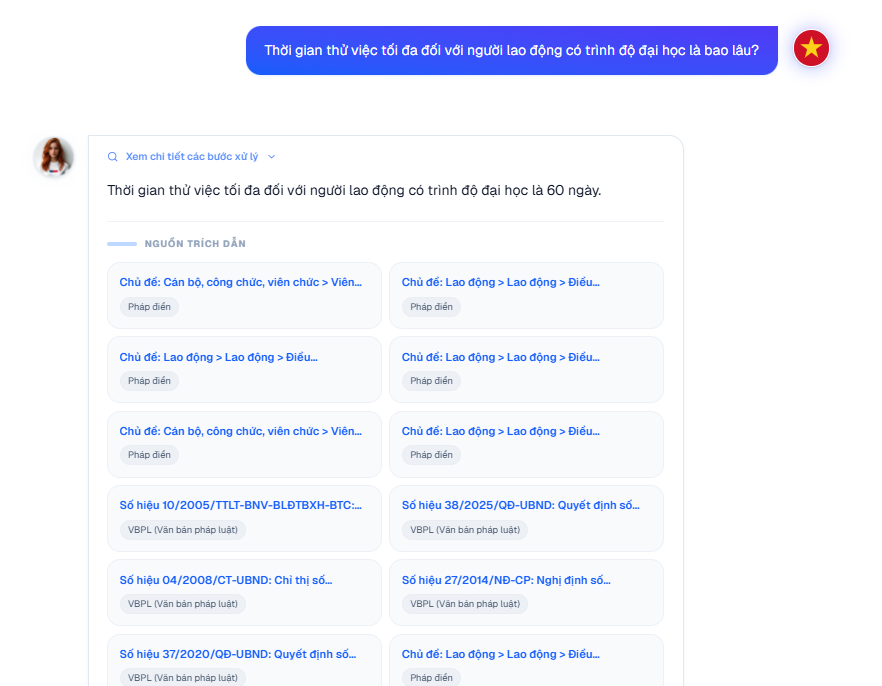
\includegraphics[width=0.65\textwidth]{pictures/chat-ui-image.png}

\refstepcounter{figure}
\textbf{Hình \thefigure:} Giao diện phản hồi câu hỏi về thời gian thử việc của hệ thống
\label{fig:chat_ui_probation}
\end{figure}

\begin{figure}[H]
\centering
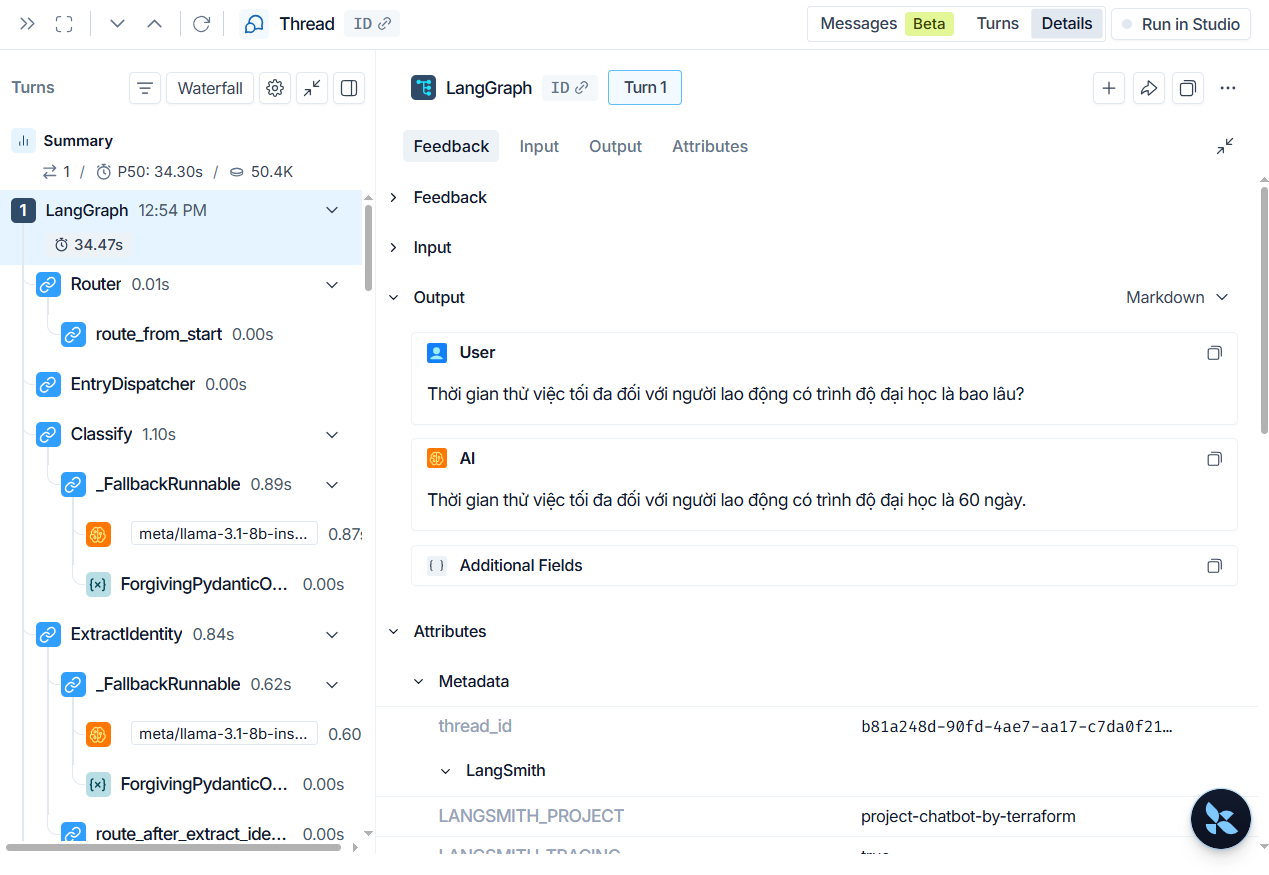
\includegraphics[width=0.65\textwidth]{pictures/langsmith-image-32.png}

\refstepcounter{figure}
\textbf{Hình \thefigure:} Chi tiết LangSmith về thời gian thử việc
\label{fig:langsmith_probation}
\end{figure}

% \newpage
% ==========================================
% Câu hỏi 2: Lực hấp dẫn
% ==========================================
% \vspace{1em}
\noindent\textbf{Câu hỏi:} Công thức tính lực hấp dẫn trong vật lý lượng tử là gì? \\
\textbf{Link:} \url{https://20206205.tech/share/d51942b0-0aff-4ead-88ae-e813c47a9a9c/2f96a259}

\begin{figure}[H]
\centering
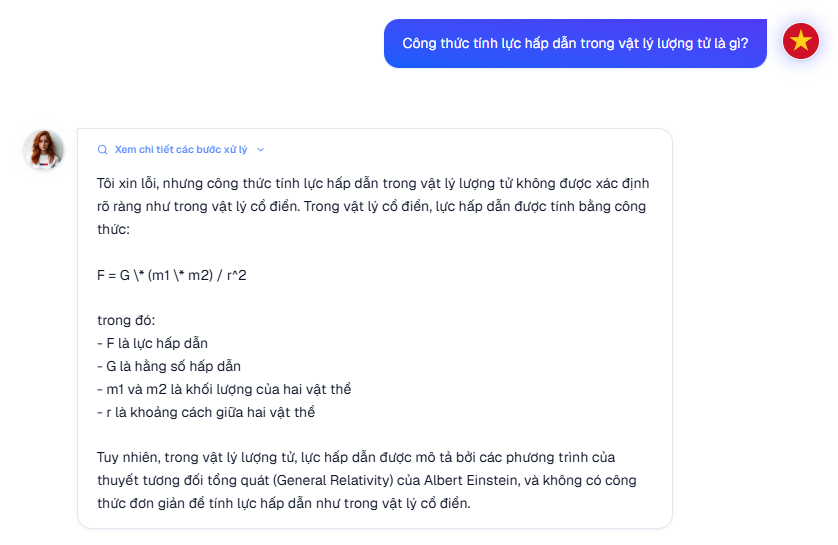
\includegraphics[width=0.65\textwidth]{pictures/chat-ui-image-1.png}

\refstepcounter{figure}
\textbf{Hình \thefigure:} Giao diện phản hồi câu hỏi về lực hấp dẫn trong vật lý lượng tử
\label{fig:chat_ui_gravity}
\end{figure}

\begin{figure}[H]
\centering
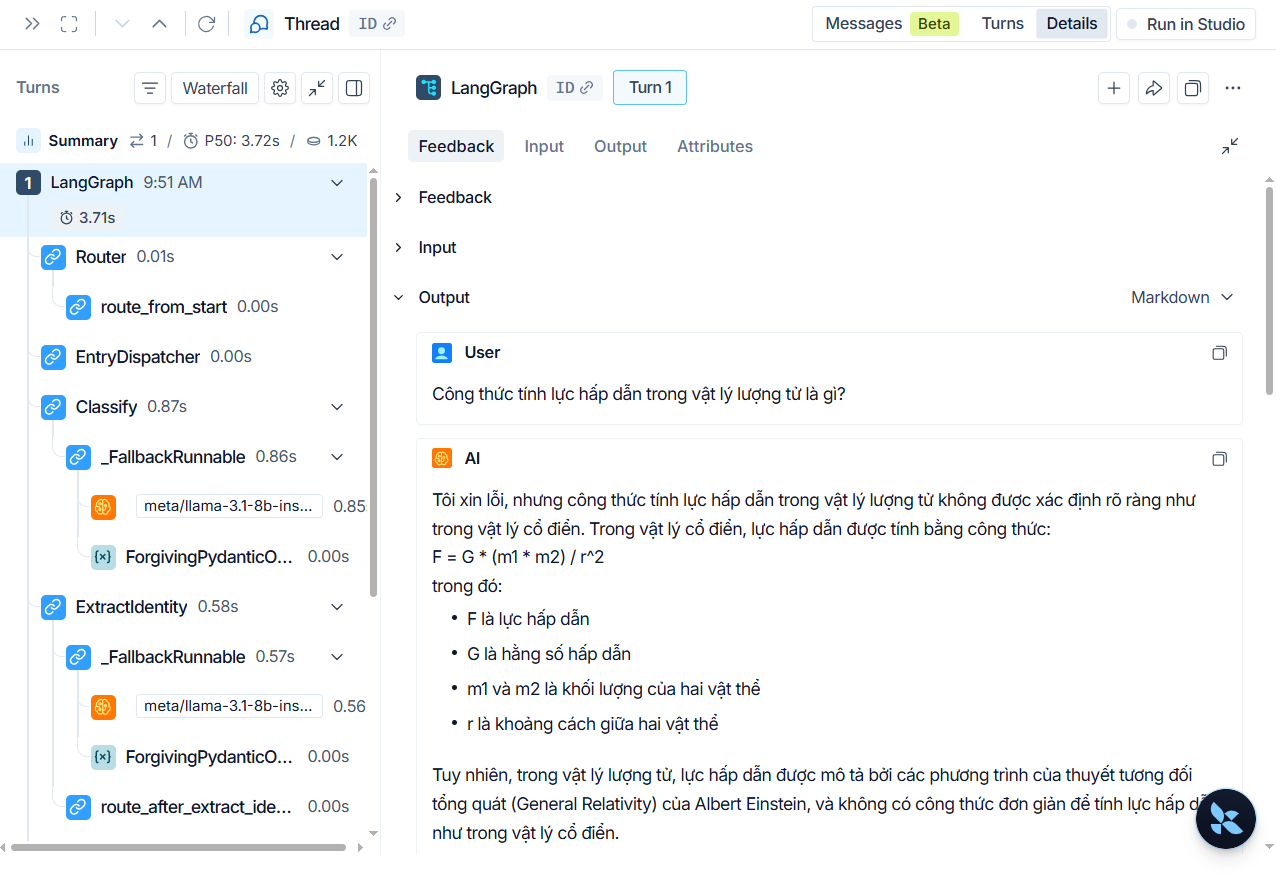
\includegraphics[width=0.65\textwidth]{pictures/langsmith-image-6.png}

\refstepcounter{figure}
\textbf{Hình \thefigure:} Chi tiết LangSmith về lực hấp dẫn
\label{fig:langsmith_gravity}
\end{figure}

% \newpage
% ==========================================
% Câu hỏi 3: Thuế thu nhập cá nhân
% ==========================================
% \vspace{1em}
\noindent\textbf{Câu hỏi:} Theo luật mới, sinh viên đi làm thêm không cần đóng thuế thu nhập cá nhân đúng không? \\
\textbf{Link:} \url{https://20206205.tech/share/0a65a3ff-e2e9-4943-920a-483fab52bfc8/eade4ab7}

\begin{figure}[H]
\centering
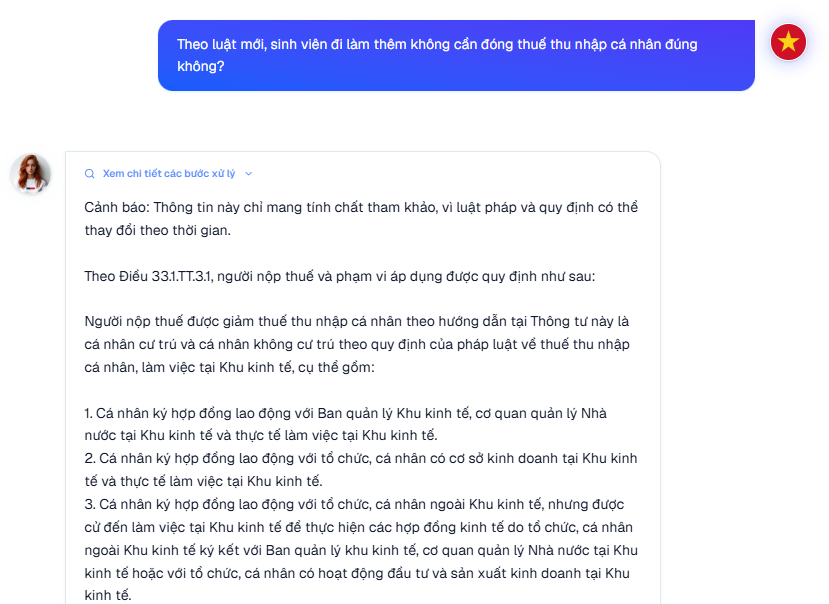
\includegraphics[width=0.65\textwidth]{pictures/chat-ui-image-4.png}

\refstepcounter{figure}
\textbf{Hình \thefigure:} Giao diện phản hồi câu hỏi về thuế thu nhập cá nhân của sinh viên đi làm thêm
\label{fig:chat_ui_tax}
\end{figure}

\begin{figure}[H]
\centering
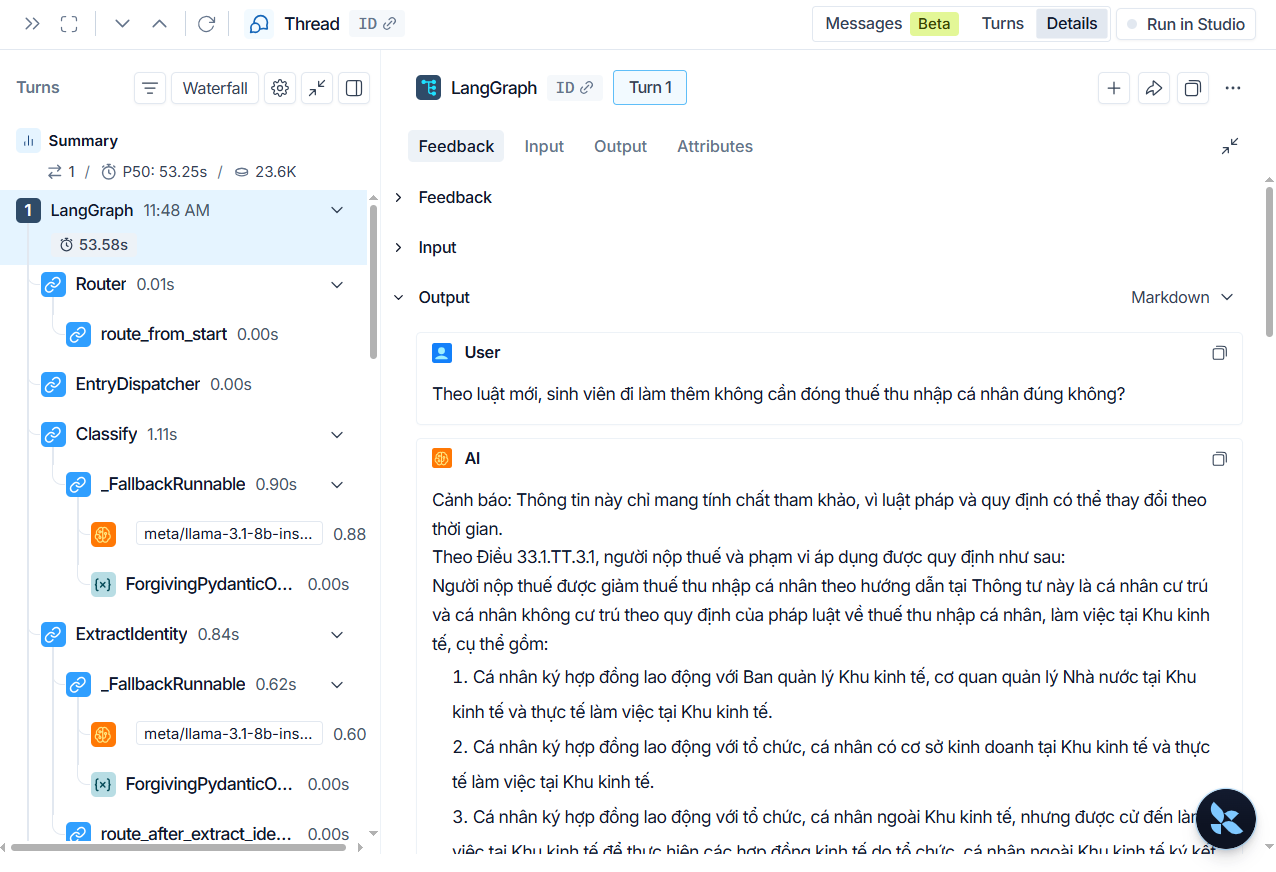
\includegraphics[width=0.65\textwidth]{pictures/langsmith-image-7.png}

\refstepcounter{figure}
\textbf{Hình \thefigure:} Chi tiết LangSmith về thuế thu nhập cá nhân
\label{fig:langsmith_tax}
\end{figure}

% \newpage
% ==========================================
% Câu hỏi 4: Đăng ký thuế
% ==========================================
% \vspace{1em}
\noindent\textbf{Câu hỏi:} Làm sao để đăng ký cái đó? \\
\textbf{Link:} \url{https://20206205.tech/share/8dc3c4e1-b63d-4d70-98f7-a89bfacefadc/2d022228}

\begin{figure}[H]
\centering
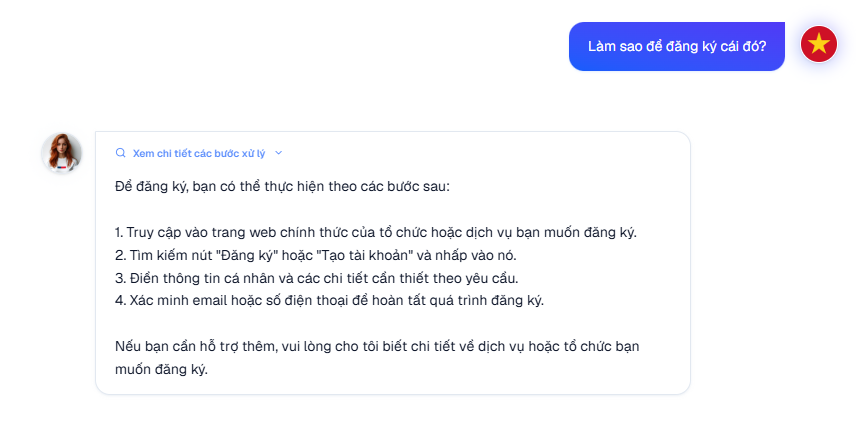
\includegraphics[width=0.9\textwidth]{pictures/chat-ui-image-2.png}

\refstepcounter{figure}
\textbf{Hình \thefigure:} Giao diện phản hồi câu hỏi tiếp nối về cách thức đăng ký
\label{fig:chat_ui_register}
\end{figure}

\begin{figure}[H]
\centering
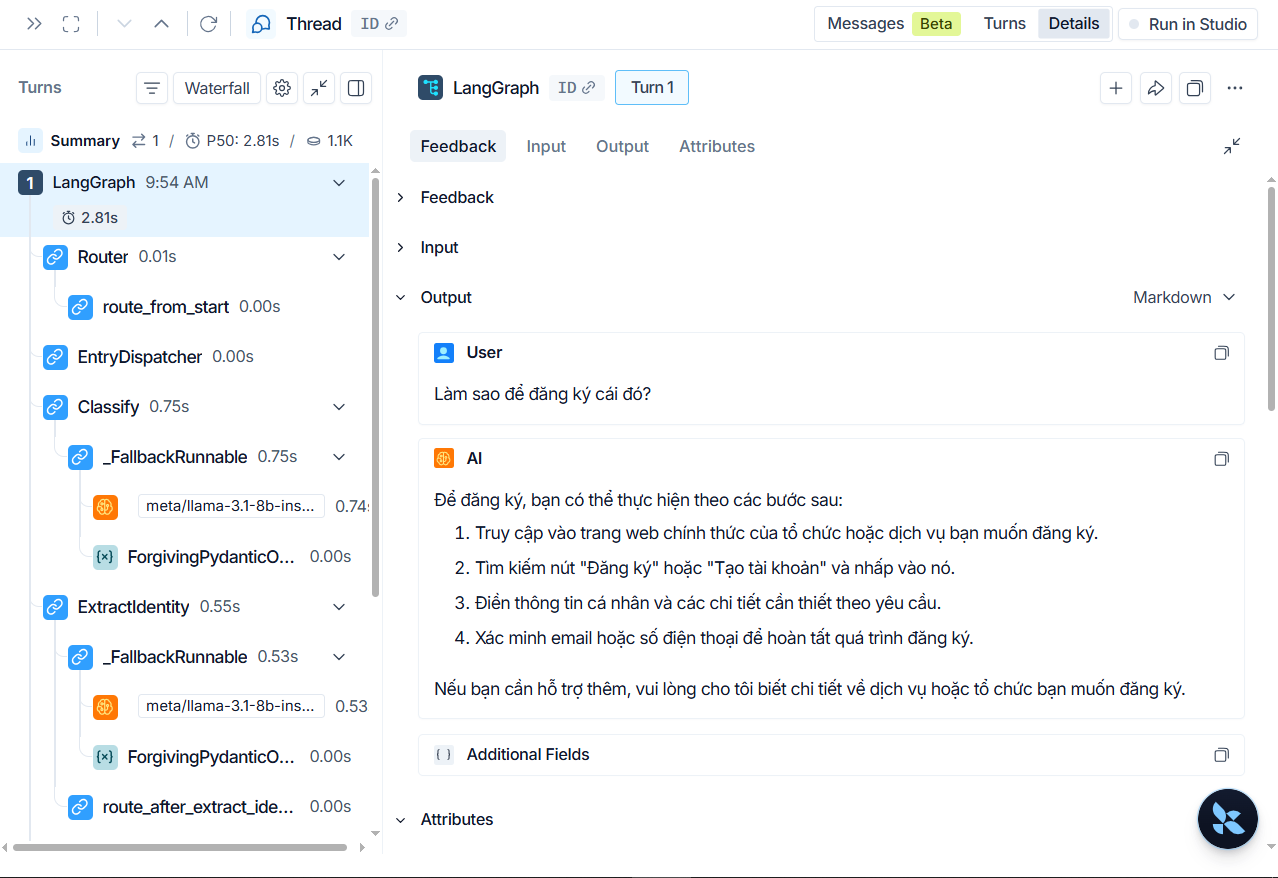
\includegraphics[width=0.65\textwidth]{pictures/langsmith-image-8.png}

\refstepcounter{figure}
\textbf{Hình \thefigure:} Chi tiết LangSmith về cách thức đăng ký
\label{fig:langsmith_register}
\end{figure}

% \newpage
% ==========================================
% Câu hỏi 5: Chấm dứt hợp đồng lao động
% ==========================================
% \vspace{1em}
\noindent\textbf{Câu hỏi:} Người lao động đơn phương chấm dứt hợp đồng lao động xác định thời hạn cần báo trước bao nhiêu ngày? \\
\textbf{Link:} \url{https://20206205.tech/share/80a989ad-6b2e-46b6-84ec-baf843c70e14/0fcaa121}

\begin{figure}[H]
\centering
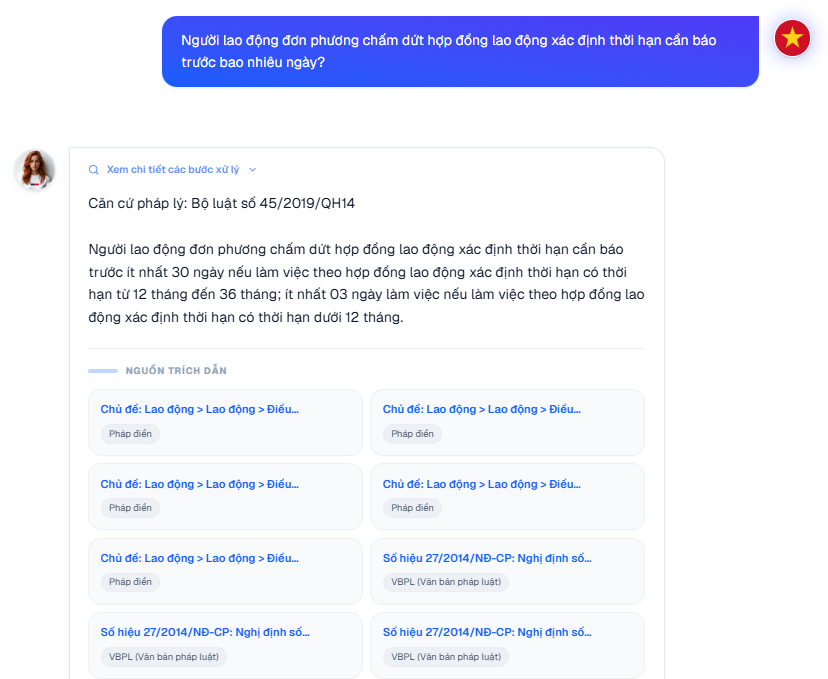
\includegraphics[width=0.65\textwidth]{pictures/chat-ui-image-5.png}

\refstepcounter{figure}
\textbf{Hình \thefigure:} Giao diện phản hồi câu hỏi về chấm dứt hợp đồng lao động
\label{fig:chat_ui_terminate_contract}
\end{figure}

\begin{figure}[H]
\centering
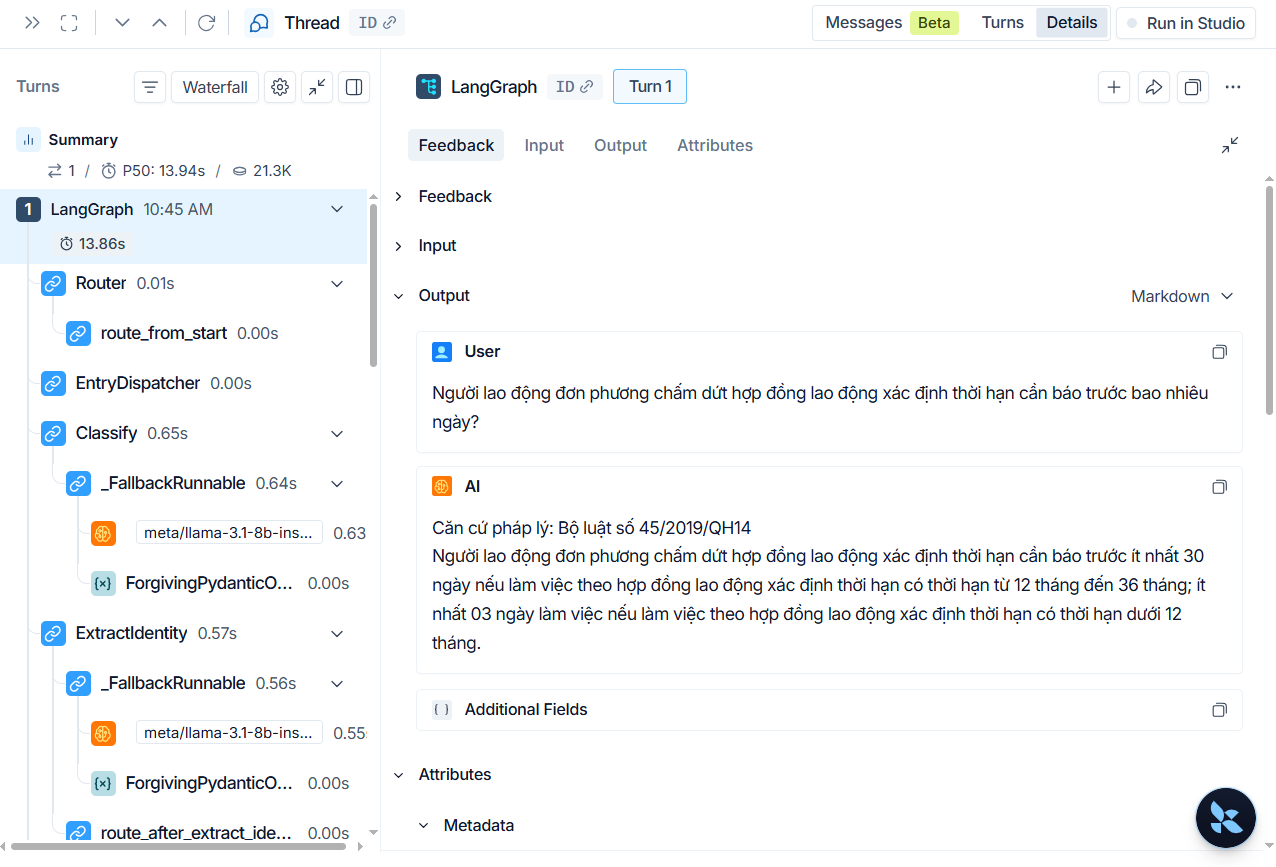
\includegraphics[width=0.65\textwidth]{pictures/langsmith-image-9.png}

\refstepcounter{figure}
\textbf{Hình \thefigure:} Chi tiết LangSmith về chấm dứt hợp đồng lao động
\label{fig:langsmith_terminate_contract}
\end{figure}
